\chapter{Preface}

I first became interested in vehicle dynamics through involvement with my college Formula SAE team.  I was on summer break after finishing my freshman year, and somehow I stumbled upon the team's website.  Racecars!  Cool!  So the next weekend, after some e-mails back and forth, I set out to a local autocross where the team was cooking burgers and hot dogs as a fundraiser.  Cars of all kinds racing through a sea of orange cones.  Having never been to an autocross before, I was curious.  ``Why is it that some cars lift the front wheel in the corners, and others lift the rear wheels?''  ``How come the real racecars don't screech tires like the street cars do?''

It didn't take long before it was clear that I had caught the racecar bug.  I was particularly drawn to suspensions.  I'm not entirely sure why that was, maybe because you could see all of the moving parts, or maybe because there was an experienced alumni who spent a lot of time in the shop who was also interested in suspension design.  Anyway, we spent many hours discussing vehicle dynamics and suspension design, pouring through the team's library of reference material and studying suspension kinematics with the help of purpose-built software.

The software we were using had terrible graphics and was somewhat tedious to use, but it provided accurate results and was simple enough to be confident that we provided the correct input.  It only permitted kinematic analysis of the suspension, and only one end of the car at a time, but it seemed well suited to our needs.  As I gained more experience and started to search for justification of more design decisions, it became clear that this software had some short comings.

%I had done some programming in high school, but hadn't really kept up

%In December 2005, I started writing software to model the dynamic response of a racecar.  I had no idea what I was getting into.  -> Didn't understand benefit of simplifying a model to gain insight into problem vs. modeling every detail of the problem. (availability of good input data - mass properties, tire data, etc.)

\begin{figure}
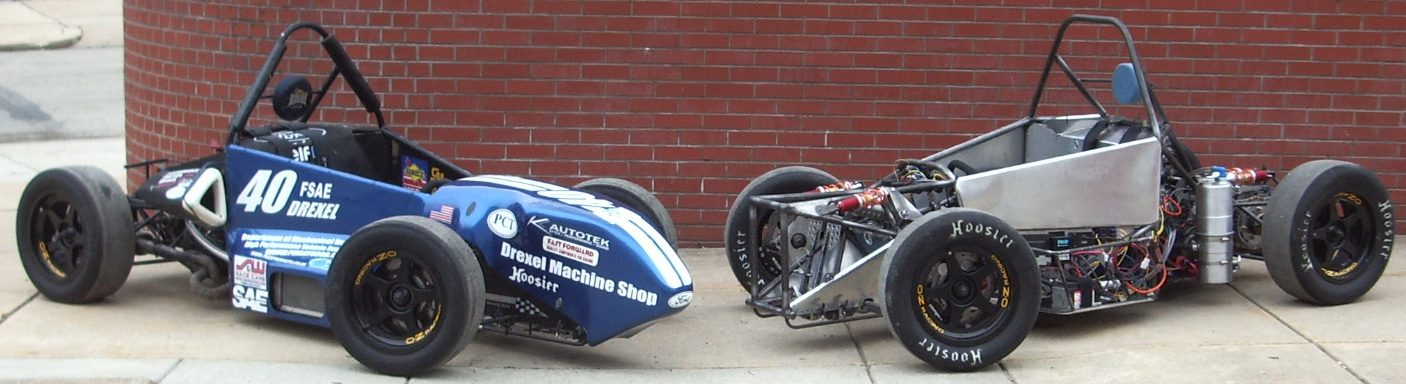
\includegraphics[width=\textwidth]{images/04-05cars}
\caption{The 2004 and (incomplete) 2005 Drexel University entries into the Formula SAE competitions}
\centering
\end{figure}